%=========================================================================

\chapter{Úvod}
V dnešních počítačových sítích dosahují přenosové rychlosti desítek gigabitů začíná se narážet na
časové limity algoritmů, jejichž účelem je zpracovávat síťová data na a sekundu
a aktuálně používané algortimy se stávají úzkým hrdlem síťových zařízení.
a začíná narážet na časové limity algoritmů, jejichž účelem je zpracovávat síťová data na
a vzniká spousta problémů se zpracování síťového provozu stávajícími technologiemi tak,
 aby nedošlo ke zdržení dat právě v zařízeních starajících se o toto zpracvování.
Tato práce se zabývá implementací která je schopna pracovat i v nejvyšších rychlostech.
Jedná se knihovna, která se skládá ze operací využívaných pro směrování dat v počítačových sítích
a jejich kontrolu na přítomnost škodlivého obsahu. Cílem knihovny je vytvořit implementaci, která bude
co možná nejrychlejší i s ohledem na paměťové nároky, jelikož síťová zař9zení na kterých může být použita
využívají různé úrovně kešování dat a při správné optimalize by nemuselo docházet k ž8dným cache-misům.

V kapitole \ref{chapter:theoretical} jsou popsány síťové modely, nad nimiž jsou operace této knihovny implementovány,
formální prostředky pro implementaci zvolených algoritmů a samotné algoritmy. Kapitola \ref{chapter:api} popisuje
veřejné rozhraní vytvořené knihovny pro operace zmíněné v kapitole \ref{chapter:theoretical},
způsoby použití a možnosti rozšíření. V kapitole \ref{chapter:results} jsou vizualizovány a popsány
výsledky implementace. Kapitola \ref{chapter:conclusion} shrnuje dosažené výsledky a nastiňuje možné směry,
kterými se může vývoj knihovny dále odvíjet.


\chapter{Teoretický rozbor}\label{chapter:theoretical}

\section{Síťové modely}

Zpracování dat síťového provozu je rozděleno do několika úrovní. Tyto úrovně jsou popsány síťovými modely.
Základním modelem je ISO/OSI, který slouží pro abstraktní rozdělení operací zpracování síťových dat a jeho použití je
pouze pro akademické účely. V reálných počítačových sítích pak dominuje model TCP/IP, který má oproti
ISO/OSI modelu menší počet vrstev.

\subsection{ISO/OSI}
ISO/OSI model je rozdělen na sedm vrstem.

\begin{enumerate}
	\item{Fyzická vrstva / Vrstva síťového rozhraní}
	\item{Linková vrstva}
	\item{Síťová vrstva}
	\item{Transportní vrstva}
	\item{Relační vrstva}
	\item{Prezentační vrstva}
	\item{Aplikační vrstva}
\end{enumerate}

\begin{figure}[!htb]
\centering
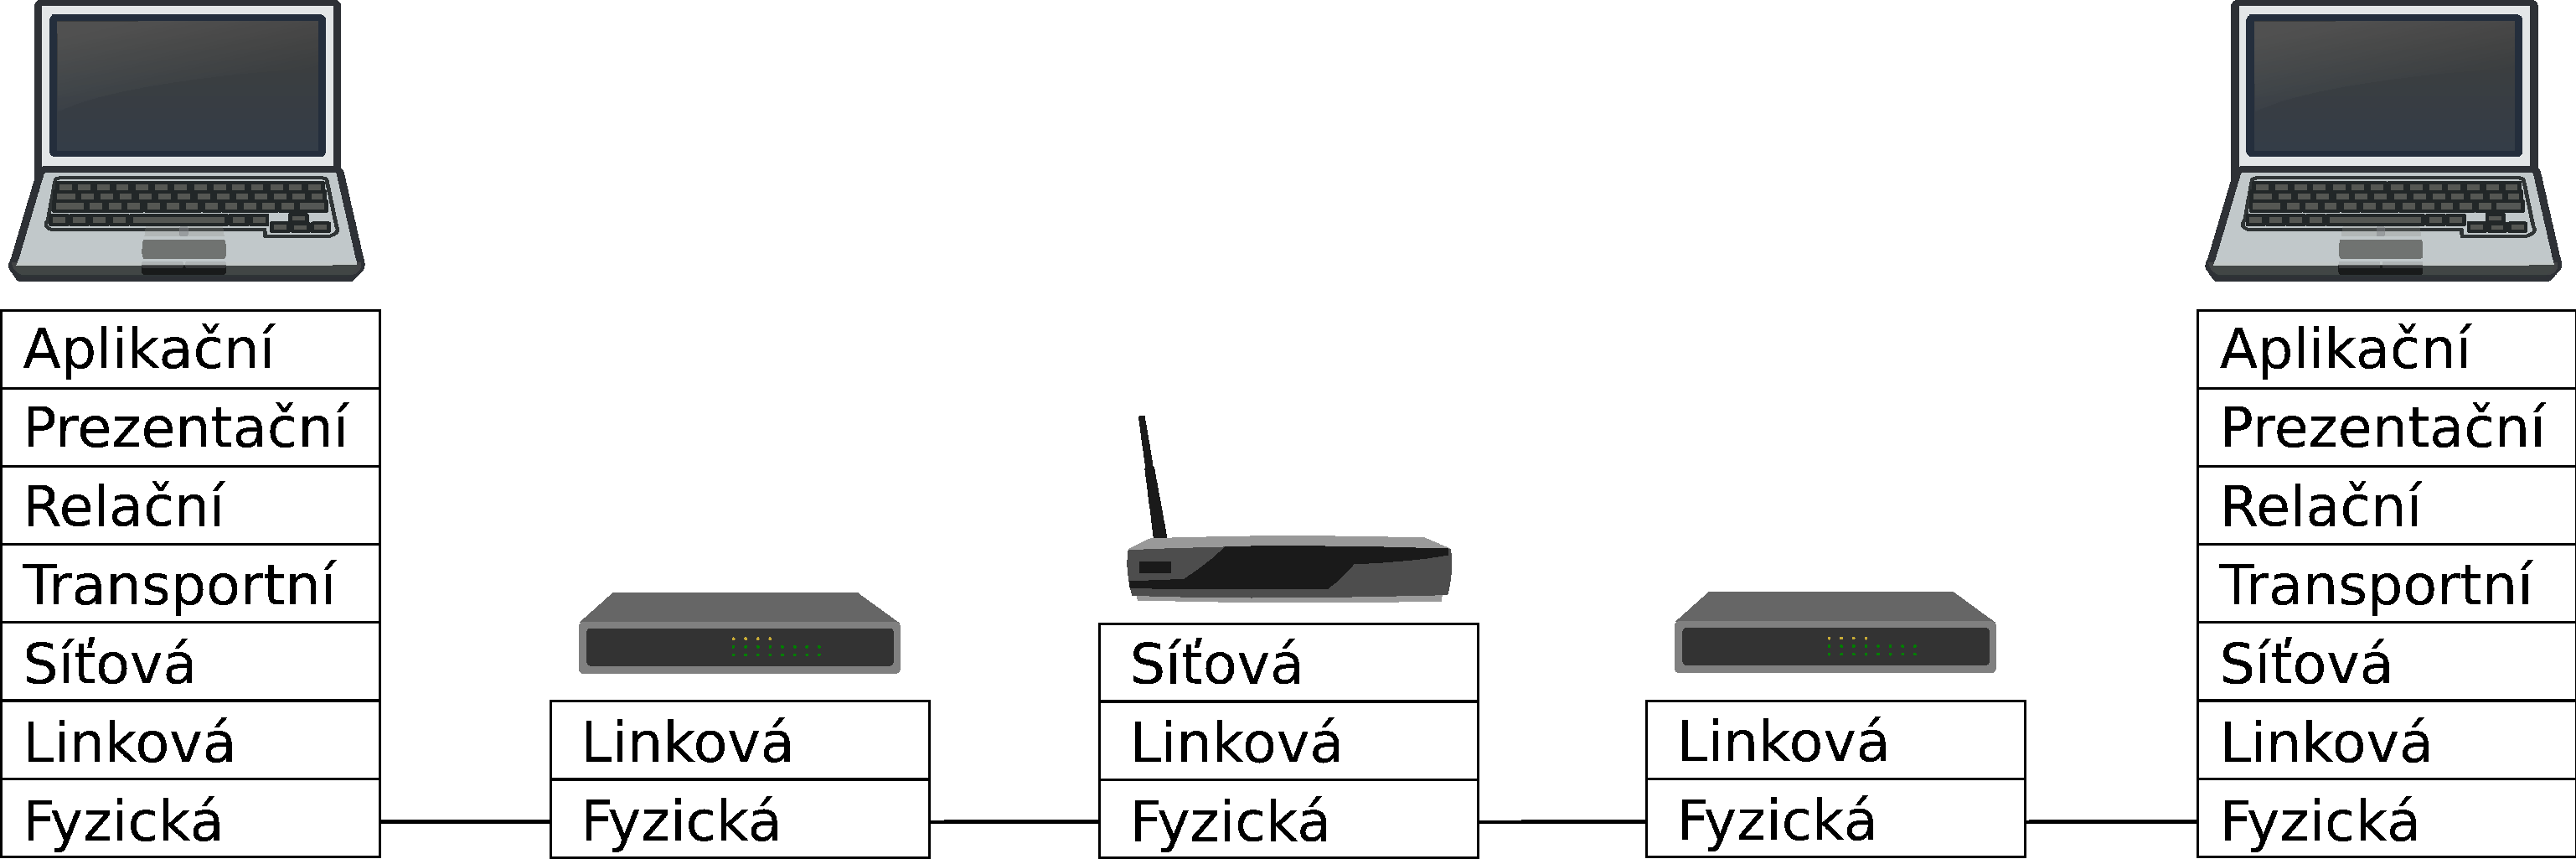
\includegraphics[scale=.25]{fig/layers.pdf}
\caption{Znázornění průchodu dat počítačovou sítí v modelu ISO/OSI}
\label{fig:layers}
\end{figure}

\subsection{TCP/IP}
TCP/IP model se skládá pouze ze čtyř vrstev.

\begin{enumerate}
	\item{Vrstva síťové rozhraní}
	\item{Síťová vrstva}
	\item{Transportní vrstva}
	\item{Aplikační vrstva}
\end{enumerate}

\subsection{Popis vrstev síťových modelů}
V následující kapitole jsou stručně popsány jednotlivé vrstvy IOS/OSI modelu,
které jsou důležité pro tuto práci.

\subsubsection{Fyzická vrstva / Vrstva síťového rozhraní}\label{layers:physical}
Nejnižší vrstva ISO/OSI modelu pracuje s daty na úrovni bitů a stará se o
jejich přenos po přenosovém médiu. Protokoly této vrstvy definují signály, které reprezentují data
a tudíž jde o protokoly implementované již v hardware síťových zařízení.

\subsubsection{Linková vrstva}\label{layers:link}
Linková vrstva je druhá nejnižší ISO/OSI modelu. Tato vrstva se stará o datovou komunikaci
obecně mezi několika uzly, které jsou přímo spojeny. Spojení může být jak fyzickým vodičem tak i
bezdrátovou technologií. Nejrozšířenější technologií pro fyzické spoje je Ethernet IEEE 802.3, pro bezdrátové spoje
je to standard IEEE 802.11. Datová jednotka na linkové vrstvě se nazývá rámec a nese v sobě kromě
zapouzdřených dat vyšších vrstev také informace o kontrolním součtu dat a adresování pomocí MAC adres.
MAC adresa je adresa fyzického zařízení, které pracuje na této vrstvě.
Adresování MAC adresou slouží pro identifikaci zařízení, které se nacházejí ve stejné počítačové síti
a za hranici této sítě se již používá IP adresace, které je vysvětleno v necházející kapitole \ref{layers:network}
Síťová zařizení pracující na této vrstvě se nazývaji switche. Úkolem switchů je zjistit MAC adresu cílové stanice a přeposlat je portem, který vede k tomuto zařízení.

\subsubsection{Síťová vrstva}\label{layers:network}
Na této vrstvě probíhá komunikace za využití IP adres. Prvky používané na této vrstvě jsou nazývaný routery.
Účelem těcho zařízení je směrování paketů procházejících sítí. K tomu využívají směrovací tabulku.
Právě pro problém vyhledání nejdelšího shodného prefixu v routovací tabulce směrovače jsou v této knihovně
implementovány dva algoritmy, \texttt{Binary search on prefix length} \ref{} a \texttt{TreeBitmap} \ref{}.
Datové struktury jsou pojmenované pakety. Pakety obsahují imformace o datovém toku a také zrojové a cílové adresy (IPv4 nebo IPv6) právě tohoto paketu.

\subsubsection{Transportní vrstva}\label{layers:transport}
Transportní vrstva pracuje s datovou strukturou zvanou segmenty.
Obsahují informace jako je kontrolní součet pro zjištění integrity dat,
pořadové číslo rámce pro spojení dat, která byla na cestě k cíli rozdělena na více částí a také obsahuje čísla portů
pro určení uživatelských aplikací, která data odeslala a která je na druhém konci má přijmout.
Na transportní vrstvě se používají dva protokoly a to TCP a UDP. UDP má nižší režii ale zase je nespolihvé.
To znamená že paket do cílového zařízení nemusí vůbec dorazit a nebo můžé dorazit v jiném pořadí než byl ze
zdrojové stanice odeslán. Situace ve kterých pozitiva jako nižší režie přebyjí zápory je hlavně přenos dat v
reálném čase. To je například streamování videa, přenost hlasu technologie VoIP a přenos informací do online her.
Spolehlivý protokol TCPzaručuje, že všechna data budou přenesena a v cílové stanici se seřadí do
stejné posloupnosti v jaké byla odeslána. Důvodem proč se data mohou rozdělit je nestabilní cesta,
po které jsou data v síti směrována. Při přenosu jednoho toku dat se může stát že se jedna cesta po které se
již poslala část dat stane nedostupnout a místo toho se data začnou směrovat přes jiná zařízení.

Zpracování dat na úrovni transportní vrstvy a všech vyšších vrstev není implementováno na síťových
zařízeních starajících se přenost dat po síti. Jediná zařízení, které implementují zpracování
dat těchto vrstev jsou koncová zařízení.

\section{Časově kritické operace}
S neustálím zvyšováním požadavků na rychlost síťového připojení také rostou nároky na rychlost
algoritmů, které na síťových zařízeních pracují. Při rychlostech, které jsou dnes reálné je problém se zpracováním
síťových operací, které mají k dispozici pouze několik desítek procesorových instrukcí pro zpracování jednoho požadavku
pokud bereme v úvahu veřejností používané procesory.

Proto v posledních letech nabírá na obrátkách trend pro využítí ASIC čipů nebo programovatelných hradlových polí.
Tyto prvky totiž umožňují rychlejší zpracování s řádově menšími požadavky.
Tohoto rychlostního rozdílu je dosaženo právě díky specializaci čípů na provádění jedné specializované operace na což jsou uzpůsobeny
narozdíl od obecných procesorů, které musejí zvládat mnohem větší repertoár operací.

\subsection{Teorie}

Pro operace hledání hledání podřetězců a zpracování regulárních výrazů popsaných v kapitolách N a N
jsou použity konečné automaty. Informace týkající se konečných automatů jsou převzaty z \cite{meduna}.

Konečný automat je uspořádaná pětice

\begin{huge}
\begin{equation}
A=(Q,\Sigma, \sigma,q_0 ,F)
\end{equation}
\end{huge}

Pro nedetermnistický konečný automat platí, že
\begin{itemize}
\item{\texttt{$Q$} je množina stavů}
\item{\texttt{$\Sigma$} je množina vstupních symbolů}
\item{\texttt{$\sigma$} je přechodová fce $Q \times \{\Sigma \cup \epsilon\} \rightarrow Q$}
\item{\texttt{$q_0 \subseteq Q$} je množina počátečních stavů}
\item{\texttt{$F \subseteq Q$} je množina konečných stavů}
\end{itemize}

Pro nedetermnistický konečný automat platí, že

\begin{itemize}
\item{\texttt{Q} je množina stavů}
\item{\texttt{$\Sigma$} je množina vstupních symbolů}
\item{\texttt{$\sigma$} je přechodová fce $Q \times \Sigma \rightarrow Q$}
\item{\texttt{$q_0 \in Q$} je počáteční stav}
\item{\texttt{$F \subseteq Q$} je množina konečných stavů}
\end{itemize}
% todo zdroj https://books.google.cz/books?id=s7gEErax71cC&vq=determinization&hl=cs&source=gbs_navlinks_s

\subsubsection{Determinizace} %todo nezobrazuje se jako nadpis
Determinizace automatu je popsána algoritmem \ref{alg:determinization}.
Při determinizace je využito dvou funkcí, první z nich je $\epsilon$-uzávěr, jehož kód je popsaný v \ref{alg:epsilon} a druhá je tzv move funkce popsaná v \ref{alg:move}

\subsubsection{Epsilon-uzávěr} %todo nezobrazuje se jako nadpis
Epsilon uzávěr je definován jako množina stavů, ze které je možné dostat se do množiny stavů pomocí přechodu
$\epsilon$.

\subsubsection{Move funkce}
Move funkce je definována jako přechod z jednoho stavu při zpracování vstupního znaku $a$.

\begin{algorithm}[H]
	\label{alg:determinization}
	\KwData{Počáteční stav nedeterministeckého automatu}
	\KwResult{Deterministický konečný automat}
	state $\leftarrow$ EpsilonClosure(nfa-start)\;
	unprocessed.push(state)\;
	created.push(state)\;
	\While{!unprocessed.empty()}
	{
		state $\leftarrow$ unprocessed.pop()\;
		\ForEach{symbol $s$ in $input\_alphabet$}
		{
			move $\leftarrow$  move(state, s)\;
			closure $\leftarrow$  EpsilonClosure(move)\;

			existing $\leftarrow$ created.find(closure)\;
			\If{!existing}
			{
				new $\leftarrow$ createState(closure)\;
				unprocessed.push(new)\;
				created.push(new)\;
			}
			\lElse
			{
				addTransition(state, existing, s)\;
			}
		}
	}
	\Return{created.first()}
	\caption{Determinize konečného automatu}
\end{algorithm}

\subsection{Regulární výrazy}

Regulární výrazy slouží pro popis operací nad jazykem.
Jazyk je je definovaný jako blah nad vstupní abecedou.
Jazek je definovaný jako iterace nad vstupní abecedou.
Iterace může  být neutrální nebo kladná.
V neutrální iteraci jazyka je oproti pozitivní iteraci zahrnut i symbol $\epsilon$,
který reprezentuje prázdný znak/řetězec.
Iterace jazyka se označuje jako $L^n$ kde \texttt{n} je označení iterace jazyka.
iterace $L^0$ obsahuje pouze jeden symbol a tím je $\epsilon$
$\epsilon$ také reprezentuje prázdný řetězec. Prázdný řetězec se může skládat z nekonečné posloupnosti $\epsilon$
Vstupní abeceda je množina symbolů.

Regulární výrazy jsou poté operace nad regulárními jazyky.
Regulární výrazy mají stejnou  vyjadřovací schopnost jako konečné automaty a pro digitální zpracování
regulárních výrazů se vždy používají konečné automaty.

Operace regulárních výrazů jsou následující

\begin{itemize}
\item{$\emptyset$ je regulární výraz reprezentující prázdnou množinu}
\item{$\epsilon$ je regulární výraz reprezentující $\{\epsilon\}$}
\item{$a, a \in \Sigma$ je regulární výraz reprezentující $\{a\}$}
\item{$(r \cdot s)$ je regulární výraz reprezentující $RS$}
\item{$(r | s)$ je regulární výraz reprezentující $R \cup S$}
\item{$(r*)$ je regulární výraz reprezentující R*}
 % todo zdroj https://books.google.cz/books?id=s7gEErax71cC&vq=determinization&hl=cs&source=gbs_navlinks_s
\end{itemize}

Znak operace konkatenace % TODO přidat referenci na item nahoře
se čast vynechává a je uvažován implicitně.

Regulární výrazy implementované v této knihovně rozšiřují množinu operací o syntaktická pozlátka

\begin{itemize}
	\item{$[abc]$ je výčet znaků, které se na vstupu mohou vyskytnout a automat je v aktuální stavu dokáže zpracovat. Je to zkrácený tvar zápisu $(a|b|c)$}
	\item{$a+$ je definováno jako pozitiní iterace, tedy $1..N$ opakování}
	\item{$a?$ je definováno jako $0..1$ iterací}
\end{itemize}

\subsection{Hledání nejdelšího prefixu}
Hledání nejdelšího shodného prefixu se používá při směrování paketů.
Pro docílení nejlepší efektivity při přeposílání paketů je nutné znát co nejpřesněji další místo, na které je paket třeba doručit.
Toho je řešeno prohledáváním routovací tabulky.
Pro dosažení větší rychlosti je routovací tabulka v paměti směrovače uložena v jiných strukturách, které tabulce neodpovídají.
V této práci jsou pro uložení routovací tabulky využity algoritmy {\tt Binary search on prefix length} a {\tt TreeBitmap}.
Oba jsou variací obecně n-árního stromu.

Při chybě alokace dojde na rozdíl od odstatních podúloh k zanechání již vytvořené fungující struktury
a to z důvodu předpokladu, že routovací tabulka se mění v čase běhu programu

\subsubsection{TreeBitmap}
\begin{algorithm}
	\KwData{tbm-root, ip, ip-length}
	\KwResult{routing rule}
	node $\leftarrow$ tbm-root\;
	position $\leftarrow$ 0\;
	\Repeat{BIT(parent.external, bits)}
	{
		bits $\leftarrow$ get-stride-bits(ip, position, prefix-length)\;
		position $\leftarrow$ position + STRIDE\;

		\If{isRule(node.internal, bits)}
		{
			longest-match = node\;
		}

		index $\leftarrow$ ones(node.external, bits)\;
		parent $\leftarrow$ node\;
		node $\leftarrow$ node.external[index]\;
	}
	\Return longest-match\;
	\caption{Hledání nejdelšího shodného prefixu algoritmem TreeBitmap}
\end{algorithm}


Z \cite{tbm} vyplívá, že je vhodné nastavit velikost střídy v rozmezí 2 - 8 bitů. Což je také rozmezí,
na které je sousředěna a otestována implementace TreeBitmap v této knihovně. Experimentálně bylo zjišténo,
že tato implementace je funkční až do velikost střídy 13bitů.

\subsubsection{Binary search on prefix length}

\begin{algorithm}
	\KwData{bspl-root, hash-table, ip, ip-length}
	\KwResult{routing rule}
	prefix-length $\leftarrow$ ip-length\;
	prefix-change $\leftarrow$ ip-length\;
	\Repeat{prefix-change > 0}
	{
		bits $\leftarrow$ get-prefix-bits(ip, prefix-length)\;
		item $\leftarrow$ hast-table.get(bits)\;
		prefix-change $\leftarrow$ prefix-change \texttt{>>} 1\;

		\If{item == NULL}{prefix-length $\leftarrow$ prefix-length - prefix-change\;}
		\ElseIf{item.type == PREFIX}{prefix-length $\leftarrow$ prefix-length + prefix-change\;}
		\lElse{break}
	}
	\lIf{item == NULL}{\Return bspl-root.default-rule}
	\caption{Hledání nejdelšího shodného prefixu algoritmem Binary search on prefix length}
\end{algorithm}


Operace vyhledání nejdelšího prefixu při využití algoritmu binary search on prefix length má časovou
složitost $\log{2}{N}$, kde \texttt{N} je počet bitů adresy. V případě IPv4 adresy je to 32 bitů a pro IPv6
adresu je to 128 bitů. Z principu algoritmu vyplívá, že nejhorší výsledky z časového hlediska bude dosahovat
při shodě prefixu, který byl zadán s lichou délkou. V tomto případě bude nutné projít všemy kroky.
Počet kroků v případě IPv4 bude 5 a v případě IPv6 adresy to pak bude 7.
Zde je vidět že i v připadě čtyřikrát delší adresy se počet kroků pro vyhledání prefixu zvedne pouze o dva,
což neplatí pro algoritmus TreeBitmap, který musí projít v nejhorším případě až čtyřikrát více
uzlů aby nalezl odpovídající prefix. Ušetřené kroky se ale nijak neprojeví na paměťové náročnosti,
protože je potřeba uchovávat stromovou strukturu pro binary search on prefix length a to z nutnosti
mít kratší prefixy v hashovací tabulce, kde dochází k rozhodnutí zda má vyhledávání směřovat k delším nebo kratším prefixům.
\cite{bspl}


\subsection{Hledání podřetězců}
Pro hledání potřetězců je implementován algoritmus autorů Aho a Corasicové. Tento algoritmus používá pro zjištění shody s podřetězcem konceptu konečného automatu. Při každé iteraci algoritmu se provede přechod o jeden znak.

\subsubsection{Aho-Corasick}
Algoritmus procházení vstupních dat je rozepsán v \ref{alg:aho} a vychází z \cite{aho}.

\begin{algorithm}
	\KwData{start-state, text}
	\KwResult{keyword}
	state = start-state\;
	\For{position $\leftarrow$ 0 \KwTo text.length}
	{
		\lWhile{goto(state, text[position]) == FAIL}{state $\leftarrow$ state.failure}
		\lIf{state.isMatch}{\Return state.keyword}
	}
	\Return NOT-MATCH\;
	\caption{Algoritmus procházení textu a hledání podřetězců}
\end{algorithm}\label{alg:aho}

Při chybě alokace se smaže celá struktura konečeného automatu, neexistuje předpoklad na dynamické přidávání pravidel za běhu programu

\subsubsection{Regulární výrazy}

\begin{figure}[!htb]
	\centering
	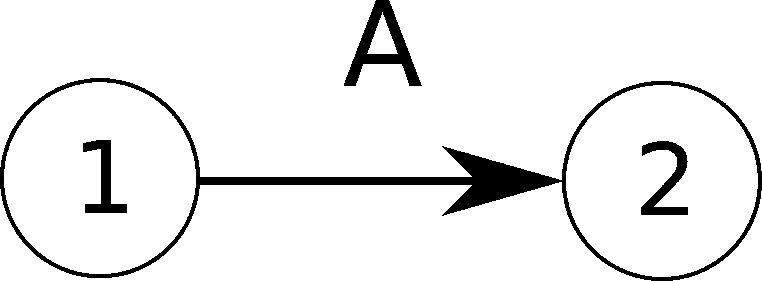
\includegraphics[scale=.25]{fig/regex-block.pdf}
	\caption{Znázornění konečného automatu reprezentujícího operaci A}
	\label{fig:regex-block}
\end{figure}

\begin{figure}[!htb]
	\centering
	\includegraphics[scale=.25]{fig/regex-concat.pdf}
	\caption{Znázornění konečného automatu reprezentujícího operaci A . B}
	\label{fig:regex-concat}
\end{figure}

\begin{figure}[!htb]
	\centering
	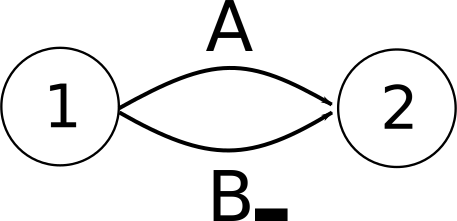
\includegraphics[scale=.25]{fig/regex-dot.pdf}
	\caption{Znázornění konečného automatu reprezentujícího operaci tečka .}
	\label{fig:regex-dot}
\end{figure}

\begin{figure}[!htb]
	\centering
	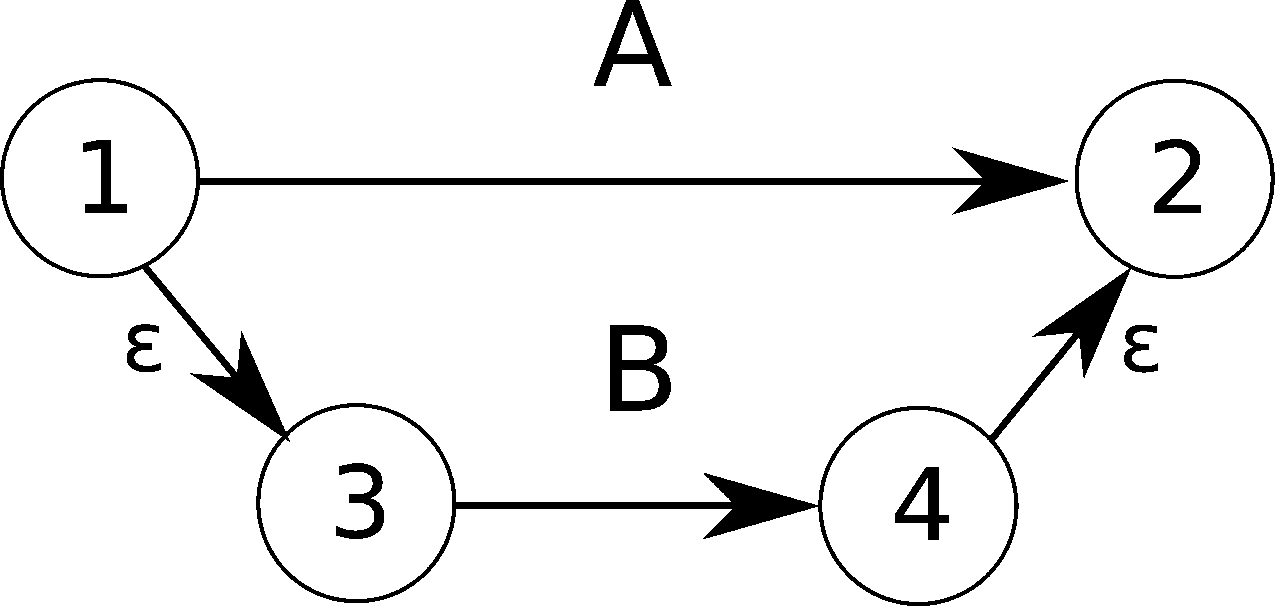
\includegraphics[scale=.25]{fig/regex-or.pdf}
	\caption{Znázornění konečného automatu reprezentujícího operaci A|B}
	\label{fig:regex-or}
\end{figure}

\begin{figure}[!htb]
	\centering
	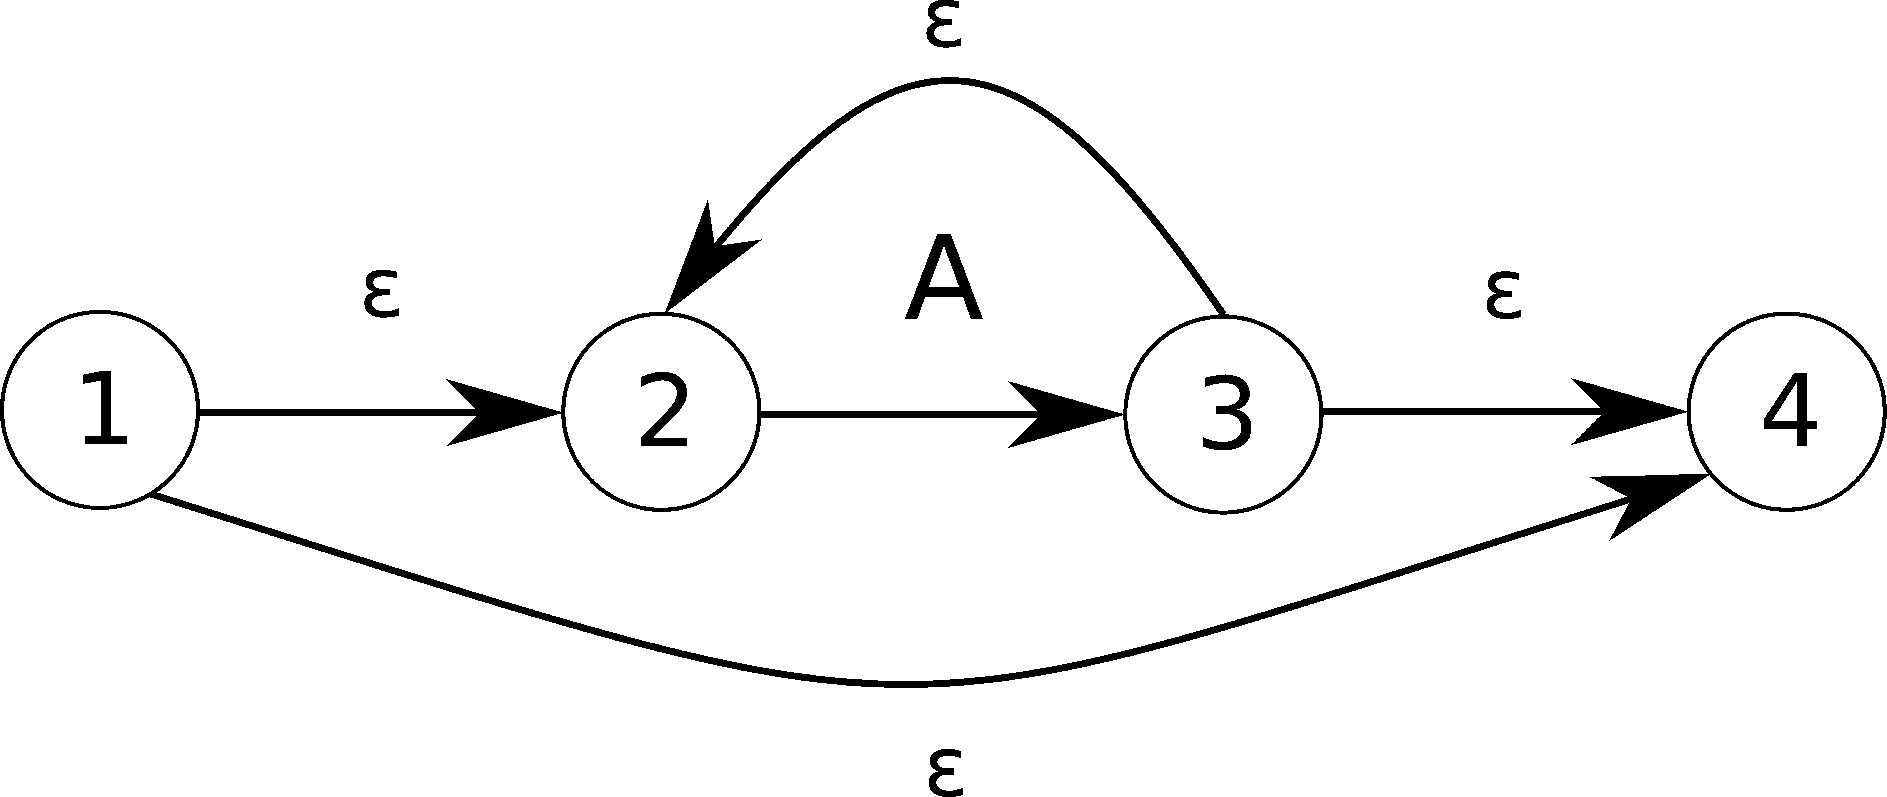
\includegraphics[scale=.25]{fig/regex-star.pdf}
	\caption{Znázornění konečného automatu reprezentujícího operaci A*}
	\label{fig:regex-star}
\end{figure}

\begin{figure}[!htb]
	\centering
	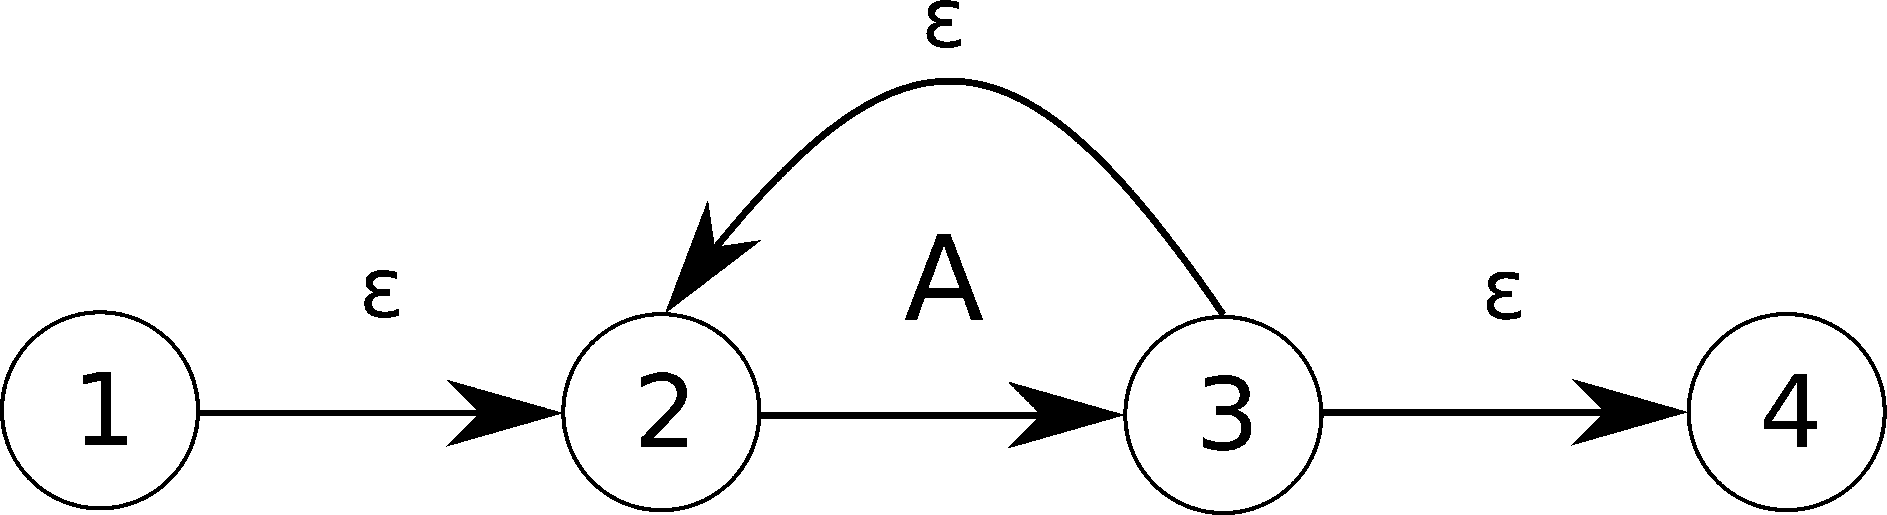
\includegraphics[scale=.25]{fig/regex-plus.pdf}
	\caption{Znázornění konečného automatu reprezentujícího operaci A+}
	\label{fig:regex-plus}
\end{figure}

\begin{figure}[!htb]
	\centering
	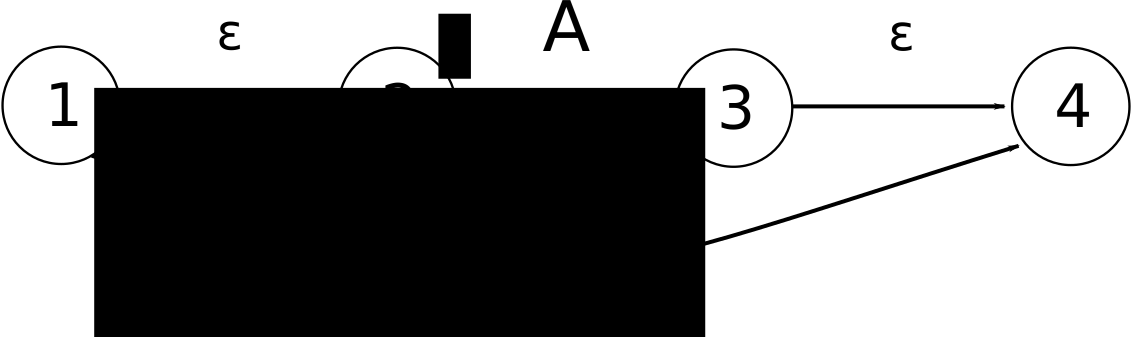
\includegraphics[scale=.25]{fig/regex-questionmark.pdf}
	\caption{Znázornění konečného automatu reprezentujícího operaci A?}
	\label{fig:regex-questionmark}
\end{figure}


Při chybě alokace se smaže celá struktura regulárního výrazu, neexistuje předpoklad na
dynamické přidávání regulárních výrazů za běhu programu.

\chapter{Návrh API knihovny}\label{chapter:api}
Knhovna \texttt{fastnet} je navržena jako množina menších knihoven, kde každá knihovna implementuje
jednu operaci používanou při zpracování síťového provozu.
Tímto návrhem je dosaženo snadné rozšiřitelnosti o další operace, jako například extrakce informací z hlaviček paketů
\i{packer header extraction} nebo klasifikace paketů \texttt{packet clasification}.
Mezi implementované operace patří vyhledání nejdelšího shodného prefix \texttt{longest prefix match} \ref{},
hledání podřetězeců \texttt{pattern matching} a regulární výrazy \texttt{regular expressions}.
Pro vyhledání nejdelšího shodného prefixu jsou implementovány algoritmy
\texttt{Binary search on prefix length}\ref{bspl} a \texttt{Tree Bitmap}\ref{tbm}.
Hledání podřetězců je implementováno algoritmem \texttt{Aho-Corasick}\ref{ac}.
Regulární výrazy jsou řešeny nedeterministickým i deterministickým konečným automatem.

Další výhodou tohoto rozdělení je možnost snadno vytvořit a používat jednotlivé podknihovny samostatně.
To se může hodit pro zařízení, která mají velmi limitované paměťové ůložiště a jejich účel
je řešit pouze jednu ze zmíněných operací.

\section{Veřejné rozhraní knihovny}
Veřejné rozhraní knihovny se skládá z veřejných rozhraní jednotlivých podknihoven.
Tyto rozhraní jsou popsány v následujících podkapitolách.

\subsection{Vyhledání nejdelšího shodného prefixu}
Pro operaci vyhledání nejdelšího shodného prefixu jsou připraveny následující funkce

% LPM IPV4 =================================================================================
\begin{Verbatim}[commandchars=\\\{\}]
\PY{n}{lpm\PYZus{}root} \PY{o}{*} \PY{n+nf}{lpm\PYZus{}init}\PY{p}{(}\PY{n}{\PYZus{}LPM\PYZus{}RULE} \PY{n}{default\PYZus{}rule}\PY{p}{)}\PY{p}{;}
\PY{k+kt}{\PYZus{}Bool} \PY{n+nf}{lpm\PYZus{}add}\PY{p}{(}\PY{n}{lpm\PYZus{}root} \PY{o}{*} \PY{n}{root}\PY{p}{,} \PY{k}{struct} \PY{n}{in\PYZus{}addr} \PY{o}{*} \PY{n}{prefix}\PY{p}{,} \PY{k+kt}{uint8\PYZus{}t} \PY{n}{prefix\PYZus{}len}\PY{p}{,} \PY{n}{\PYZus{}LPM\PYZus{}RULE} \PY{n}{rule}\PY{p}{)}\PY{p}{;}
\PY{k+kt}{void} \PY{n+nf}{lpm\PYZus{}update}\PY{p}{(}\PY{n}{lpm\PYZus{}root} \PY{o}{*} \PY{n}{root}\PY{p}{,} \PY{k}{struct} \PY{n}{in\PYZus{}addr} \PY{o}{*} \PY{n}{prefix}\PY{p}{,} \PY{k+kt}{uint8\PYZus{}t} \PY{n}{prefix\PYZus{}len}\PY{p}{,} \PY{n}{\PYZus{}LPM\PYZus{}RULE} \PY{n}{rule}\PY{p}{)}\PY{p}{;}
\PY{k+kt}{void} \PY{n+nf}{lpm\PYZus{}remove}\PY{p}{(}\PY{n}{lpm\PYZus{}root} \PY{o}{*} \PY{n}{root}\PY{p}{,} \PY{k}{struct} \PY{n}{in\PYZus{}addr} \PY{o}{*} \PY{n}{prefix}\PY{p}{,} \PY{k+kt}{uint8\PYZus{}t} \PY{n}{prefix\PYZus{}len}\PY{p}{)}\PY{p}{;}
\PY{k+kt}{void} \PY{n+nf}{lpm\PYZus{}destroy}\PY{p}{(}\PY{n}{lpm\PYZus{}root} \PY{o}{*} \PY{n}{root}\PY{p}{)}\PY{p}{;}
\PY{n}{\PYZus{}LPM\PYZus{}RULE} \PY{n+nf}{lpm\PYZus{}lookup}\PY{p}{(}\PY{n}{lpm\PYZus{}root} \PY{o}{*} \PY{n}{root}\PY{p}{,} \PY{k}{struct} \PY{n}{in\PYZus{}addr} \PY{o}{*} \PY{n}{key}\PY{p}{)}\PY{p}{;}
\end{Verbatim}

%LPM IPV6 =================================================================================
\begin{Verbatim}[commandchars=\\\{\}]
\PY{n}{lpm6\PYZus{}root} \PY{o}{*} \PY{n+nf}{lpm6\PYZus{}init}\PY{p}{(}\PY{n}{\PYZus{}LPM\PYZus{}RULE} \PY{n}{default\PYZus{}rule}\PY{p}{)}\PY{p}{;}
\PY{k+kt}{\PYZus{}Bool} \PY{n+nf}{lpm6\PYZus{}add}\PY{p}{(}\PY{n}{lpm6\PYZus{}root} \PY{o}{*} \PY{n}{root}\PY{p}{,} \PY{k}{struct} \PY{n}{in6\PYZus{}addr} \PY{o}{*} \PY{n}{prefix}\PY{p}{,} \PY{k+kt}{uint8\PYZus{}t} \PY{n}{prefix\PYZus{}len}\PY{p}{,} \PY{n}{\PYZus{}LPM\PYZus{}RULE} \PY{n}{rule}\PY{p}{)}\PY{p}{;}
\PY{k+kt}{void} \PY{n+nf}{lpm6\PYZus{}update}\PY{p}{(}\PY{n}{lpm6\PYZus{}root} \PY{o}{*} \PY{n}{root}\PY{p}{,} \PY{k}{struct} \PY{n}{in6\PYZus{}addr} \PY{o}{*} \PY{n}{prefix}\PY{p}{,} \PY{k+kt}{uint8\PYZus{}t} \PY{n}{prefix\PYZus{}len}\PY{p}{,} \PY{n}{\PYZus{}LPM\PYZus{}RULE} \PY{n}{rule}\PY{p}{)}\PY{p}{;}
\PY{k+kt}{void} \PY{n+nf}{lpm6\PYZus{}remove}\PY{p}{(}\PY{n}{lpm6\PYZus{}root} \PY{o}{*} \PY{n}{root}\PY{p}{,} \PY{k}{struct} \PY{n}{in6\PYZus{}addr} \PY{o}{*} \PY{n}{prefix}\PY{p}{,} \PY{k+kt}{uint8\PYZus{}t} \PY{n}{prefix\PYZus{}len}\PY{p}{)}\PY{p}{;}
\PY{k+kt}{void} \PY{n+nf}{lpm6\PYZus{}destroy}\PY{p}{(}\PY{n}{lpm6\PYZus{}root} \PY{o}{*} \PY{n}{root}\PY{p}{)}\PY{p}{;}
\PY{n}{\PYZus{}LPM\PYZus{}RULE} \PY{n+nf}{lpm6\PYZus{}lookup}\PY{p}{(}\PY{n}{lpm6\PYZus{}root} \PY{o}{*} \PY{n}{root}\PY{p}{,} \PY{k}{struct} \PY{n}{in6\PYZus{}addr} \PY{o}{*} \PY{n}{key}\PY{p}{)}\PY{p}{;}
\end{Verbatim}

Proměnné datových typů \texttt{lpm\_root} a \text{lpm6\_root} reprezentují právě jeden kořen
všech datových struktur. Tím je možné odlišit několik routovací tabulek.

\subsection{Hledání podřetězců}
Pro hledání podřetězců jsou implementovány následující funkce.

%PM API =================================================================================
\begin{Verbatim}[commandchars=\\\{\}]
\PY{n}{pm\PYZus{}root} \PY{o}{*} \PY{n+nf}{pm\PYZus{}init}\PY{p}{(}\PY{p}{)}\PY{p}{;}
\PY{k+kt}{\PYZus{}Bool} \PY{n+nf}{pm\PYZus{}match}\PY{p}{(}\PY{n}{pm\PYZus{}root} \PY{o}{*} \PY{n}{root}\PY{p}{,} \PY{k+kt}{char} \PY{o}{*} \PY{n}{input}\PY{p}{,} \PY{k+kt}{unsigned} \PY{n}{length}\PY{p}{,} \PY{n}{pm\PYZus{}result} \PY{o}{*} \PY{n}{result}\PY{p}{)}\PY{p}{;}
\PY{k+kt}{\PYZus{}Bool} \PY{n+nf}{pm\PYZus{}match\PYZus{}next}\PY{p}{(}\PY{n}{pm\PYZus{}result} \PY{o}{*} \PY{n}{result}\PY{p}{)}\PY{p}{;}
\PY{k+kt}{\PYZus{}Bool} \PY{n+nf}{pm\PYZus{}add}\PY{p}{(}\PY{n}{pm\PYZus{}root} \PY{o}{*} \PY{n}{root}\PY{p}{,} \PY{n}{pm\PYZus{}keyword} \PY{n}{keywords}\PY{p}{[}\PY{p}{]}\PY{p}{,} \PY{k+kt}{unsigned} \PY{n}{size}\PY{p}{)}\PY{p}{;}
\PY{k+kt}{void} \PY{n+nf}{pm\PYZus{}destroy}\PY{p}{(}\PY{n}{pm\PYZus{}root} \PY{o}{*} \PY{n}{root}\PY{p}{)}\PY{p}{;}
\PY{k+kt}{\PYZus{}Bool} \PY{n+nf}{pm\PYZus{}remove}\PY{p}{(}\PY{n}{pm\PYZus{}root} \PY{o}{*} \PY{n}{root}\PY{p}{,} \PY{k+kt}{char} \PY{o}{*} \PY{n}{text}\PY{p}{,} \PY{k+kt}{unsigned} \PY{n}{length}\PY{p}{)}\PY{p}{;}
\end{Verbatim}

Proměnné datového typ \texttt{pm\_root} a reprezentují právě jeden kořen konečného automatu a
díky tomu je možné uchovávat několik odlišných strktur sloužících každá pro jiné účely.

Hledání podřetězců \texttt{pm\_match} skončí svůj průchod konečný automatem v momentě nálezu první shody
s libovolným podřetězcem zadaným při volání \texttt{pm\_add}. Vpřípadě, že není nalezena žádná shoda
se vstupními podřetězci je vrácen výsledek \texttt{false}.

Čtvrtým parametrem funkce \texttt{pm\_match} může být \texttt{NULL} nebo odkaz na datovou strukturu
\texttt{pm\_result}. V případě \texttt{NULL} argumentu již nelze procházet textem a hledat další shody.
Pokud je zadán odkaz na existující strukturu \texttt{pm\_result} je možné procházet celým textem a ukládat
všechny nalezené shody s podřetězci. Jednotlivé položky struktury \texttt{pm\_result} jsou.

% PM_RESULT =================================================================================
\begin{Verbatim}[commandchars=\\\{\}]
\PY{k}{typedef} \PY{k}{struct}
\PY{p}{\PYZob{}}
	\PY{n}{PM\PYZus{}RULE} \PY{o}{*} \PY{n}{rule}\PY{p}{;}
	\PY{k+kt}{unsigned} \PY{n}{size}\PY{p}{;}
	\PY{k+kt}{unsigned} \PY{n}{count}\PY{p}{;}
	\PY{k+kt}{unsigned} \PY{n}{position}\PY{p}{;}
	\PY{k+kt}{char} \PY{o}{*} \PY{n}{input}\PY{p}{;}
	\PY{k+kt}{unsigned} \PY{n}{length}\PY{p}{;}
	\PY{n}{\PYZus{}ac\PYZus{}state} \PY{o}{*} \PY{n}{state}\PY{p}{;}
\PY{p}{\PYZcb{}} \PY{n}{pm\PYZus{}result}\PY{p}{;}
\end{Verbatim}

Pro použití programátorem jsou určeny pouze položky

\begin{itemize}
	\item{count - počet nalezených pravidel}
	\item{position - pozice v textu, na které došlo k první shodě}
	\item{rule - pole s uloženými čísly vyhovujících pravidel}
\end{itemize}

Pro uložení výsledků procházení textu je možné používat různé struktury typu \texttt{pm\_result}
a je jen na programátory konkrétní aplikace jaký postup zvolí.
V knihovně \texttt{pm} jsou implementováný funkce pro vytvoření a zničení této struktury.

% PM_RESULTAPI =================================================================================
\begin{Verbatim}[commandchars=\\\{\}]
\PY{n}{pm\PYZus{}result} \PY{o}{*} \PY{n+nf}{pm\PYZus{}result\PYZus{}init}\PY{p}{(}\PY{p}{)}\PY{p}{;}
\PY{k+kt}{void} \PY{n+nf}{pm\PYZus{}result\PYZus{}destroy}\PY{p}{(}\PY{n}{pm\PYZus{}result} \PY{o}{*} \PY{n}{result}\PY{p}{)}\PY{p}{;}
\end{Verbatim}


Pro vkládání podřetězců je vytvořena vlastní datová sturktura, a pole těchto struktur je předáváno do funkce
\texttt{pm\_add}. Důvodem pro tuto implementaci namísto přidávání jednotlivých podřetězců samostatně
je relativně časově náročné procházení stavového automatu a generování tzv. failure přechodů,
které je nutné provést po každé změně datové struktury.

% PM_KEYWORD =================================================================================
\begin{Verbatim}[commandchars=\\\{\}]
\PY{k}{typedef} \PY{k}{struct}
\PY{p}{\PYZob{}}
	\PY{k+kt}{char} \PY{o}{*} \PY{n}{content}\PY{p}{;}
	\PY{k+kt}{unsigned} \PY{n}{length}\PY{p}{;}
	\PY{n}{PM\PYZus{}RULE} \PY{n}{rule}\PY{p}{;}
\PY{p}{\PYZcb{}} \PY{n}{pm\PYZus{}keyword}\PY{p}{;}
\end{Verbatim}


\subsection{Regulární výrazy}
Knihovna \texttt{regex} implementující regulární výrazy nabízí dvě možnosti pro procházení
vstupních dat a to deterministický \texttt{dfa} a nedeterministický konečný automat \texttt{nfa}.
Z toho důvodu jsou odlišeny všechny funkce dle typu konečného automatu, který je použit.
Oproti hledání nejdelšího shodného prefixu \ref{} nejsou tyto implementace od sebe odlišeny
různými soubory neboť deterministické automaty vycházejí z nedeterministický a pouze používají
determinizaci.

Pro nedeterministické konečné automaty to jsou následující funkce.

% REGEX NFA =================================================================================
\begin{Verbatim}[commandchars=\\\{\}]
\PY{n}{regex\PYZus{}nfa} \PY{o}{*} \PY{n+nf}{regex\PYZus{}construct\PYZus{}nfa}\PY{p}{(}\PY{n}{regex\PYZus{}pattern} \PY{n}{patterns}\PY{p}{[}\PY{p}{]}\PY{p}{,} \PY{k+kt}{unsigned} \PY{n}{count}\PY{p}{)}\PY{p}{;}
\PY{k+kt}{int} \PY{n+nf}{regex\PYZus{}match\PYZus{}nfa}\PY{p}{(}\PY{n}{regex\PYZus{}nfa} \PY{o}{*} \PY{n}{root}\PY{p}{,} \PY{k+kt}{char} \PY{o}{*} \PY{n}{input}\PY{p}{,} \PY{k+kt}{unsigned} \PY{n}{length}\PY{p}{)}\PY{p}{;}
\PY{k+kt}{void} \PY{n+nf}{regex\PYZus{}destroy\PYZus{}nfa}\PY{p}{(}\PY{n}{regex\PYZus{}nfa} \PY{o}{*} \PY{n}{root}\PY{p}{)}\PY{p}{;}
\end{Verbatim}

Pro deterministické konečné automaty jsou to tyto funkce.
% REGEX DFA =================================================================================
\begin{Verbatim}[commandchars=\\\{\}]
\PY{n}{regex\PYZus{}dfa} \PY{o}{*} \PY{n+nf}{regex\PYZus{}construct\PYZus{}dfa}\PY{p}{(}\PY{n}{regex\PYZus{}pattern} \PY{n}{patterns}\PY{p}{[}\PY{p}{]}\PY{p}{,} \PY{k+kt}{unsigned} \PY{n}{count}\PY{p}{)}\PY{p}{;}
\PY{k+kt}{int} \PY{n+nf}{regex\PYZus{}match\PYZus{}dfa}\PY{p}{(}\PY{n}{regex\PYZus{}dfa} \PY{o}{*} \PY{n}{root}\PY{p}{,} \PY{k+kt}{char} \PY{o}{*} \PY{n}{input}\PY{p}{,} \PY{k+kt}{unsigned} \PY{n}{length}\PY{p}{)}\PY{p}{;}
\PY{k+kt}{void} \PY{n+nf}{regex\PYZus{}destroy\PYZus{}dfa}\PY{p}{(}\PY{n}{regex\PYZus{}dfa} \PY{o}{*} \PY{n}{root}\PY{p}{)}\PY{p}{;}
\end{Verbatim}

Pro vytvoření regulárních výrazů je podobně jako u hledání podřetězců \ref{}
použita pomocná struktura \texttt{regex\_pattern}, která je předávána do funkcí \texttt{regex\_[nfa|dfa]\_construct}.
Výsledný konečný automat, ať už deterministický nebo nedeterministický je výsledek spojení jednotlivých
konečných automatů pro každý regulární výraz. Tím je umožněna detekce shody několika
regulární výrazů v jednom průchodu vstupními daty i s přesnou identifikací jaký regulární
výraz se shoduje se vstupními daty. To je také jedním z důvodů proč nejsou použity regulární výrazy ze standardní
knihovny jazyka C.
Další důvody pro vlastní implementaci regulární výrazů je možnost zvolit nejvhodnější algoritmus pro danou operaci.
Mějme na paměti že determinizací může dojít až k exponenciální nárustu stavů konečného automatu, což může problém
zvláště při použití specializovaných HW implementací, kde je možno narazit na paměťové limity.
Dalším důvodem je převod implementace do akcelerovaného hardware.

%REGEX PATTERN =================================================================================
\begin{Verbatim}[commandchars=\\\{\}]
\PY{k}{typedef} \PY{k}{struct}
\PY{p}{\PYZob{}}
	\PY{k+kt}{unsigned} \PY{n}{length}\PY{p}{;}
	\PY{k+kt}{unsigned} \PY{k+kt}{char} \PY{n}{id}\PY{p}{;}
	\PY{k+kt}{char} \PY{o}{*} \PY{n}{input}\PY{p}{;}
\PY{p}{\PYZcb{}} \PY{n}{regex\PYZus{}pattern}\PY{p}{;}
\end{Verbatim}

\begin{figure}[!htb]
	\centering
	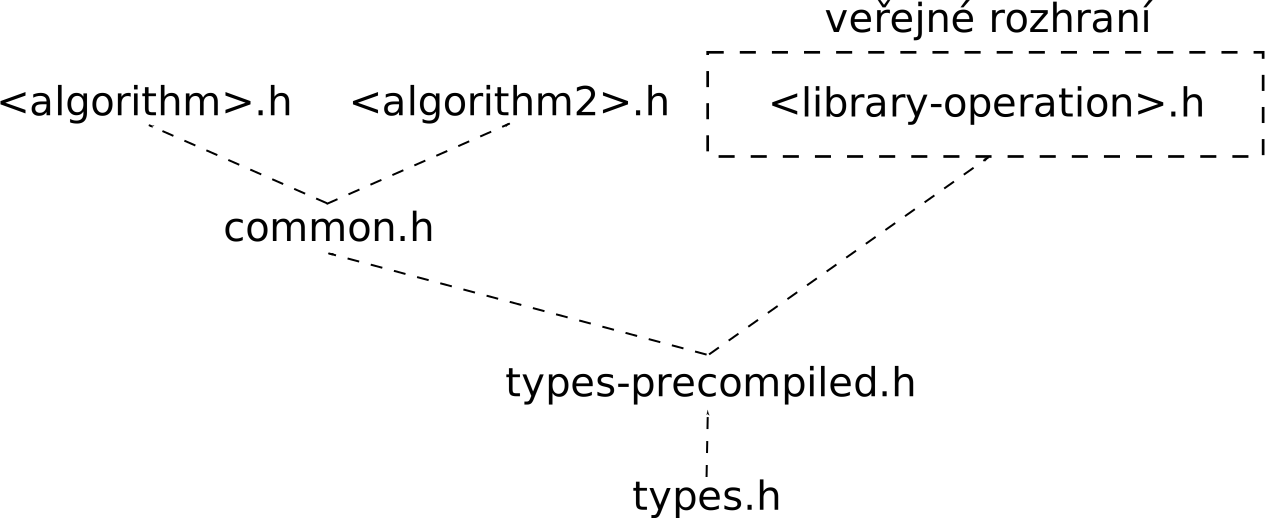
\includegraphics[scale=.25]{fig/header-dependencies.pdf}
	\caption{Diagram závislostí hlavičkových souborů}
	\label{fig:header-dependecies}
\end{figure}

hlavičkové soubory jsou rozděleny na veřejné a privátní rozhraní, kde privátní rozhraní je používáno pouze uvnitř knihovny. Hierarchickou strukturu je možné vidět na obrázku \ref{fig:header-dependecies}.

Jako výchozí hlavičkový soubor je použit types.h, který obsahuje definice datových struktur pro všechny algoritmy v podknihovně, které musí být viditelné i z veřejného rozhraní. Dalším souborem je types-precompiled.h, který je generován z types.h při překladu když se vybírá používaný algoritmus. common.h je hlavičkový soubor společný pro všechny algoritmy v podknihovně a algortihm.h pak obsahuje deklarace právě pro jeden konkrétní algoritmus.
sublib.h je pak hlavičkový soubor, který tvoří veřejné rozhraní ke knihovním funkcím.

\subsection{Použití knihovny}
Celou knihovnu je možné sestavit příkazem \texttt{make all} v hlavním adresáři knihovny.
Při tomto příkazu bude celá knihovna sestavena s definovaným NDEBUG, což má za následek vypuštění všech
volání funkce assert, která slouží pro ověřovaní správné funkčnosti.

Dalšími cíly pro program \texttt{make} jsou

\begin{itemize}
	\item{\texttt{test} - spustí automatické testování všech částí knihovny}
	\item{\texttt{bech} - spustí benchmarky všech částí knihovny}
	\item{\texttt{clean} - smaže všechny soubory vytvořené překladem}
\end{itemize}

\subsection{Rošíření knihovny}

Pro rozšíření knihovny je nutné přidat knihovnu implementující danou operaci
do adresáře \texttt{lib/src} a upravit příslušný soubor \texttt{Makefile} v daném adresáři.
Dále je vhodné vytvořit testovací program a sadu testů, kterou je možné automatizovaně spouštět a vyhodnocovat.
Tyto soubory pak umístit do adresáře \texttt{lib/test/<operace>}.
Další vhodnou součástí knihovny operace je benchmark pro vyhodnocení rychlosti/paměťové náročnosti jednotlivých
implementací dané operace.


\chapter{Výsledky}\label{chapter:results}

\section{Hledání nejdelšího shodného prefixu}
U algoritmu bspl je doba vyhledání prefixu velice závislá na velikosti hešovací tabulky a proto je vhodné odhadnout počet záznamů tabulky alespoň řádově a dle toho pak nastavit velikost konstantu {\tt \_HTABLE\_SIZE} v souboru bspl.h na hodnotu, která alespoň řádově odpovídá předpodkládané velikosti hešovací tabulky.

\begin{figure}[!htb]
\centering
\includegraphics[scale=1]{fig/lpm-ipv4.pdf}
\caption{Benchmark pro IPv4}
\label{fig:lpm-ipv4}
\end{figure}

\begin{figure}[!htb]
\centering
\includegraphics[scale=1]{fig/lpm-ipv6.pdf}
\caption{Benchmark pro IPv6}
\label{fig:lpm-ipv4}
\end{figure}

\chapter{Závěr}\label{chapter:conclusion}
Závěrečná kapitola obsahuje zhodnocení dosažených výsledků se zvlášť vyznačeným vlastním přínosem studenta. Povinně se zde objeví i zhodnocení z pohledu dalšího vývoje projektu, student uvede náměty vycházející ze zkušeností s řešeným projektem a uvede rovněž návaznosti na právě dokončené projekty.

%=========================================================================

\section{Další vývoj knihovny}

V následujících krocích tvorby knihovny \texttt{fastnet} bude vhodné implementovat operace
navržené v kapitole \ref{} s alespoň jedním algoritmem pro každou z uvedených operací.

Dále je možné provést optimalizace jednotlivých algoritmů z pohledu jak paměťové tak i časové náročnosti.

\subsection{Optimalizace}
U implementace \texttt{Binary search on prefix length} je možné rozdělit strukturu \texttt{\_bspl\_node}
na dvě a to jednu pro každou verzi IP protokolu. Tím se dosáhne snížení paměťové náročnosti
pro každý uzel o 12B.

Další optimalizací je přepsání leaf-pushing do iterativní průchod za použití morrisova algoritmu.

Dále je možné spojit položky \texttt{type} a \texttt{prefix\_length} struktury \texttt{\_bspl\_node}
do jednoho byte. To je možné z důvodu rozsahu \texttt{prefix\_length} $1-128$ a pouze dvou typů uzlu,
což je možné reprezentovat jedním bytem.

\subsection{Stress-testing}
- ověřit že se knihovna chová dle specifikace i při nedostaku paměti a v případech, kdy dojde k malloc nullu
a provolávají se různé funkce
